\chapter{Hasil dan Pembahasan}
Bab ini akan menjelaskan hasil dari metode yang telah dijelaskan pada bab sebelumnya. 
Pembahasan akan dibagi berdasarkan fitur yang dikembangkan, dan akan menjelaskan mengenai hasil dari proses desain gamifikasi, hasil dari pengembangan aplikasi, dan proses pengujiannya masing masing.
Selanjutnya dijelaskan juga mengenai pengujian keseluruhan aplikasi dengan melibatkan pengguna nyata atau responden.

\section{Hasil Pengembangan Desain Gamifikasi}
Gamifikasi yang diimplementasikan merupakan elemen gamifikasi untuk domain pembelajaran \textit{Declarative Knowledge}.
Dengan demikian elemen utama dari desain ini ialah pengembangan pemebalajaran yang akan diimplementasikan menjadi sebuah fitur materi yang disusun berurutan, dan sebuah kuis yang dapat dikerjakan berulang ulang.
Pengembangan gamifikasinya sendiri menggunakan \textit{Framework MDA} dimana kerangka kerja ini mengimplementasikan mekanika permainan, dinamika permainan, dan estetika permainan ke dalam aplikasi pembalajran ini.

Warna yang digunakan dalam desain aplikasi ini menggunakan warna utama hijau.
Hijau dipilih karena memberika kesan kesagaran dan kesehatan.
Pemilihan warna yang tepat untuk konteks pembelajaran merupakan upaya untuk memenuhi elemen estetika permainan untuk menarik pengguna menggunakan aplikasinya.  A
plikasi ini dinamai "\textbf{MedQ}" untuk kesan \textit{simple} da mudah diingat. MedQ adalah kependekan dari \textit{Medical Education Quiz}.
\subsection{\textit{FeatureSet : Sign-In}}
\begin{figure}[H]
	\centering
	\begin{subfigure}[b]{0.23\textwidth}
		\centering
	  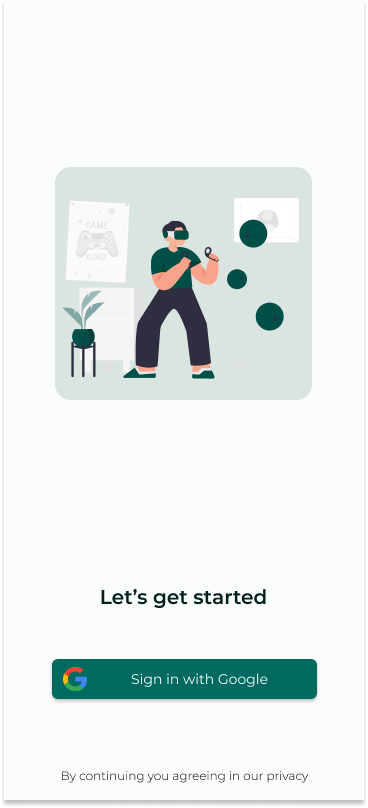
\includegraphics[width=\linewidth]{contents/chapter-3/images/HF-login.png}
	  \caption{\textit{Light Mode}}
	  \label{fig:HasilLogin}
	\end{subfigure}
	\begin{subfigure}[b]{0.23\textwidth}
		\centering
	  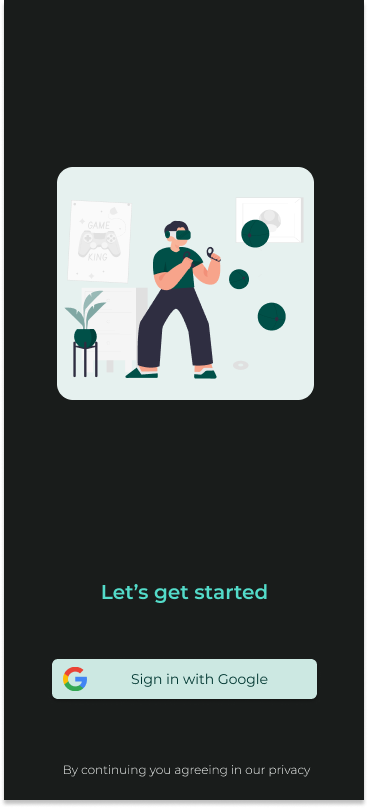
\includegraphics[width=\linewidth]{contents/chapter-3/images/HF-login-dt.png}
	  \caption{\textit{Dark Mode}}
	  \label{fig:HasilLogin2}
	\end{subfigure}
	\caption{\textit{Prototype} antarmuka halaman \textit{Log-in}}
	\label{Fig:HasilFeatureSetLogin}
\end{figure}
Fitur ini menghasilkan 2 desain, yaitu desain halaman login untuk mode terang, dan mode gelap sebagaimana yang dicantumkan pada gambar \ref*{Fig:HasilFeatureSetLogin}.
Fitur ini hanya menampilkan 1 tombol yang berfungsi untuk meminta akses ke aplikasi dengan autentikasi google.
% ============================================
\subsection{\textit{Feature set : Dashboard}}
\begin{figure}[H]
	\centering
	\begin{subfigure}[b]{0.23\textwidth}
		\centering
	  
\includegraphics[width=\linewidth]{contents/chapter-3/images/HF-Boarding.png}
	  \caption{Halaman utama}
	  \label{fig:HasilBoarding}
	\end{subfigure}
	\begin{subfigure}[b]{0.23\textwidth}
		\centering
	  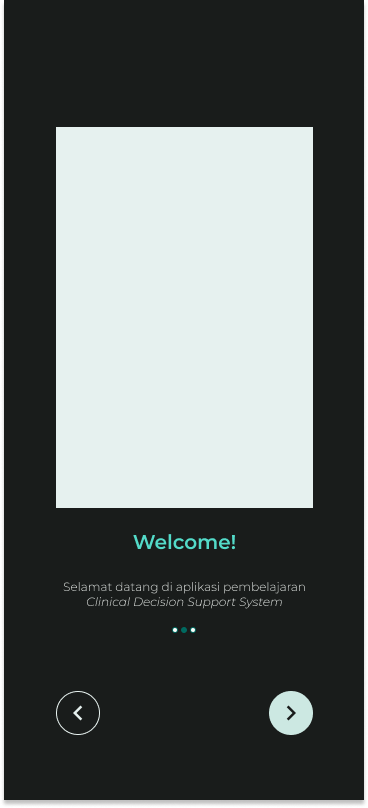
\includegraphics[width=\linewidth]{contents/chapter-3/images/HF-Boarding-dt.png}
	  \caption{\textit{Warning dialog}}
	  \label{fig:HasilBoarding2}
	\end{subfigure}
	\caption{\textit{Prototype} antarmuka halaman \textit{On Boarding}}
	\label{Fig:HasilFeatureSetBoarding}
\end{figure}
Fitur \textit{On Boarding} didesain seperti pada gambar \ref*{Fig:HasilFeatureSetBoarding}. Halaman ini akan ditampilkan jika pengguna belum pernah \textit{Sign-in}.
\begin{figure}[H]
	\centering
	\begin{subfigure}[b]{0.23\textwidth}
		\centering
	  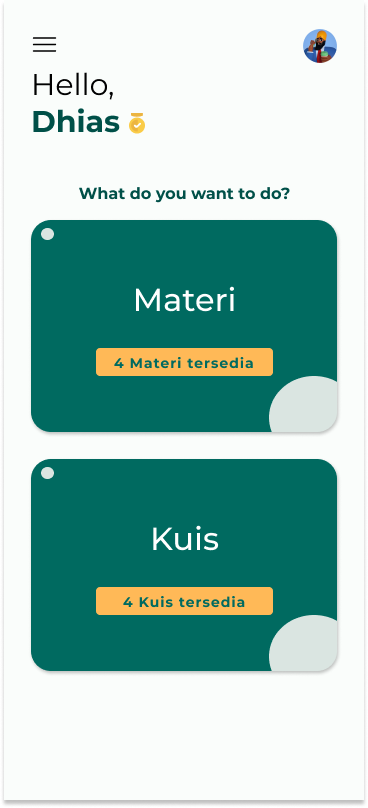
\includegraphics[width=\linewidth]{contents/chapter-3/images/HF-Main.png}
	  \caption{Halaman utama}
	  \label{fig:HasilMainDash}
	\end{subfigure}
	\begin{subfigure}[b]{0.23\textwidth}
		\centering
	  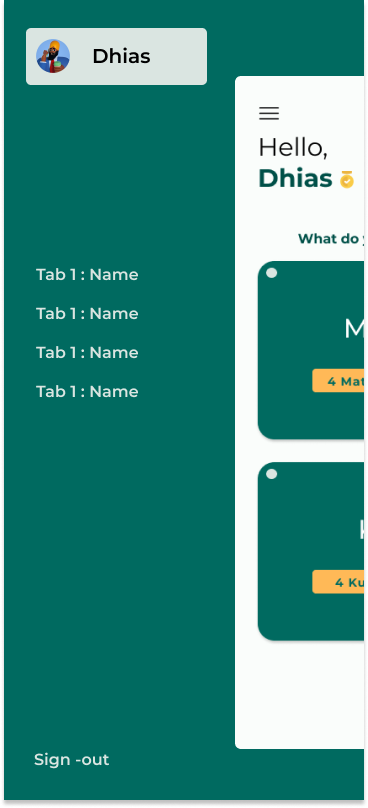
\includegraphics[width=\linewidth]{contents/chapter-3/images/HF-Drawer.png}
	  \caption{\textit{Drawer}}
	  \label{fig:HasilMainDash2}
	\end{subfigure}
	\begin{subfigure}[b]{0.23\textwidth}
		\centering
	  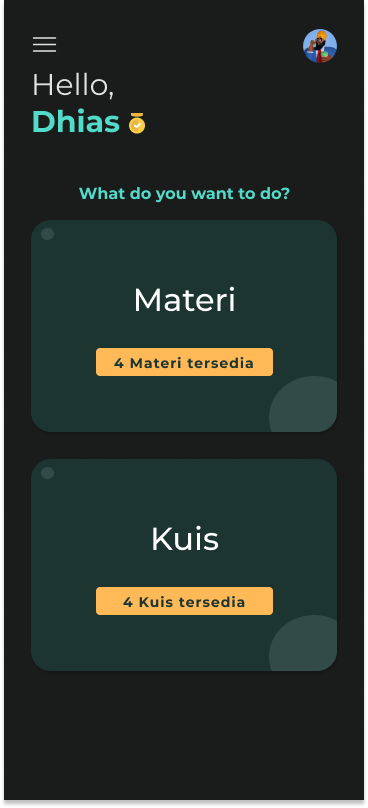
\includegraphics[width=\linewidth]{contents/chapter-3/images/HF-Main-dt.png}
	  \caption{Halaman Utama}
	  \label{fig:HasilMainDash-dark}
	\end{subfigure}
    \begin{subfigure}[b]{0.23\textwidth}
		\centering
	  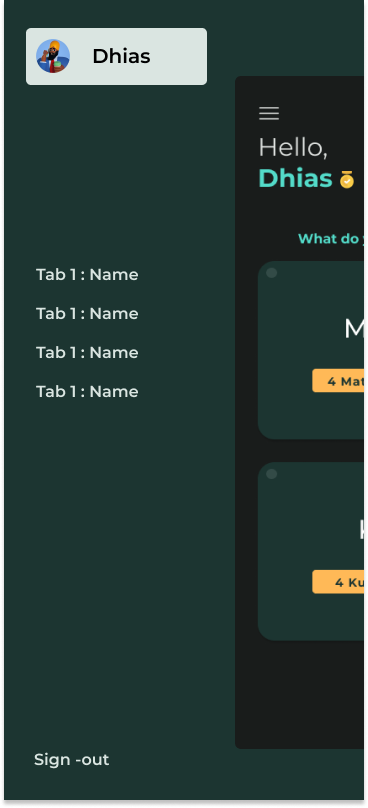
\includegraphics[width=\linewidth]{contents/chapter-3/images/HF-Drawer-dt.png}
	  \caption{\textit{Drawer}}
	  \label{fig:HasilMainDash2-dark}
	\end{subfigure}
	\caption{\textit{Prototype} antarmuka halaman \textit{Dashboard} utama}
	\label{Fig:HasilFeatureDashboard}
\end{figure}
Setalah \textit{On Boarding}, desain selanjutnya pada fitur set ini adalah fitur halaman utama atau \textit{dashboard}. Gambar ditampilkan pada gambar \ref*{Fig:FeatureSetDashboard}.
Fitur ini menjadi fitur navigasi awal untuk pergi ke fitur-fitur lainnya.
\subsection{\textit{Feature set} : Kuis}
\begin{figure}[H]
	\centering
	\begin{subfigure}[b]{0.23\textwidth}
		\centering
	  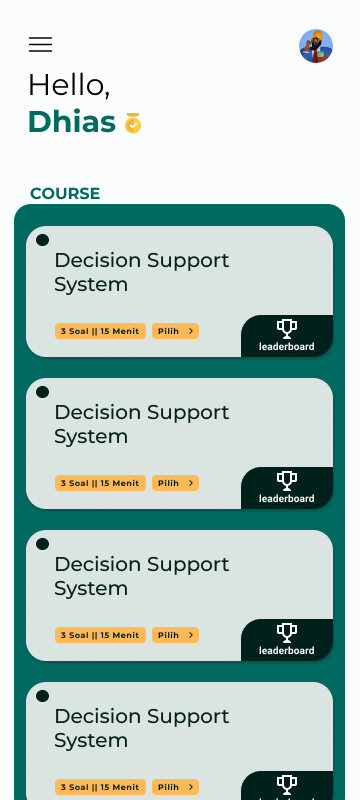
\includegraphics[width=\linewidth]{contents/chapter-3/images/HF-QuizList.png}
	  \caption{\textit{Light Mode}}
	  \label{fig:HasilQuizList}
	\end{subfigure}
	\begin{subfigure}[b]{0.23\textwidth}
		\centering
	  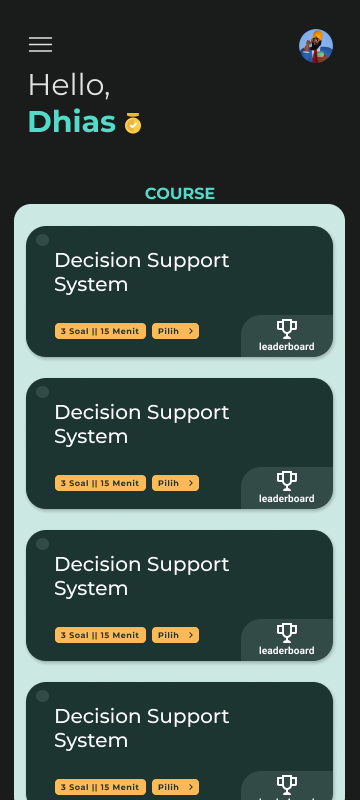
\includegraphics[width=\linewidth]{contents/chapter-3/images/HF-QuizList-dt.png}
	  \caption{\textit{Dark Mode}}
	  \label{fig:HasilQuizList2}
	\end{subfigure}
	\caption{\textit{Prototype} antarmuka halaman daftar kuis}
	\label{Fig:HasilFeatureSetQuizListt}
\end{figure}
Fitur ini adalah fitur utama dari implementasi mekanika permainan dalam aplikasi ini. Gambar \ref*{Fig:HasilFeatureSetQuizListt} adalah desain halaman fitur daftar kuis yang tersedia.
\begin{figure}[H]
	\centering
	\begin{subfigure}[b]{0.23\textwidth}
		\centering
	  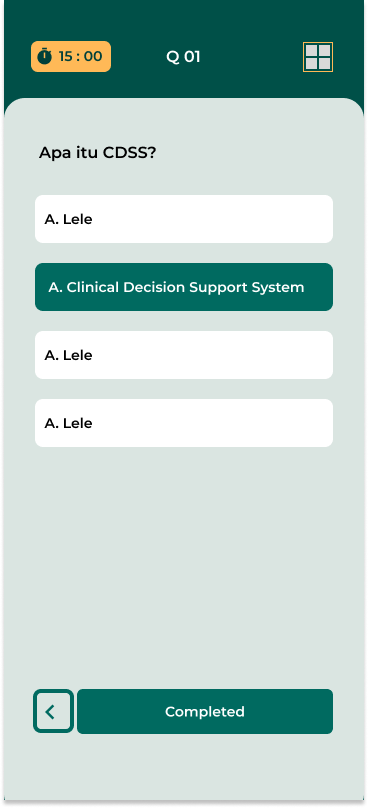
\includegraphics[width=\linewidth]{contents/chapter-3/images/HF-kuis1.png}
	  \caption{Jawab kuis}
	  \label{fig:midFi-login}
	\end{subfigure}
	\begin{subfigure}[b]{0.23\textwidth}
		\centering
	  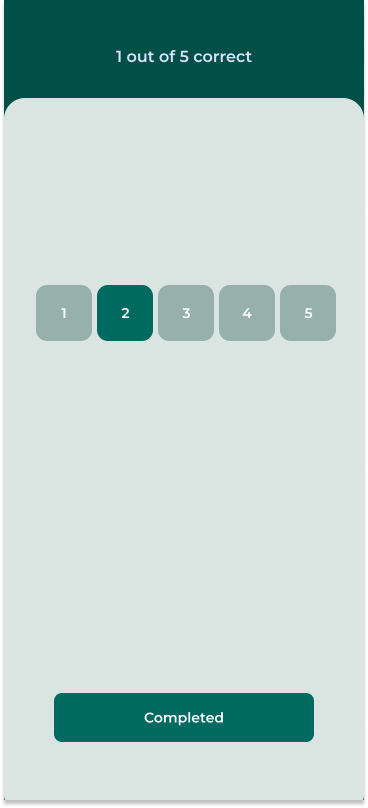
\includegraphics[width=\linewidth]{contents/chapter-3/images/HF-kuis2.png}
	  \caption{\textit{overview}}
	  \label{fig:pilihNomor}
	\end{subfigure}
	\begin{subfigure}[b]{0.23\textwidth}
		\centering
	  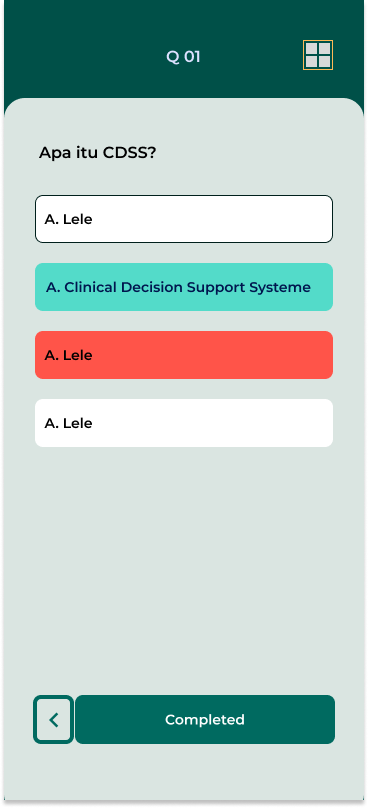
\includegraphics[width=\linewidth]{contents/chapter-3/images/HF-kuis3.png}
	  \caption{\textit{Review}}
	  \label{fig:subjectScreen}
	\end{subfigure}
	\caption{\textit{Prototype} antarmuka halaman kuis mode terang}
	\label{Fig:HasilFeatureSetQuiz}
\end{figure}
Gambar \ref*{Fig:FeatureSetQuiz} adalah desain halaman kuis mode terang. 
Fitur kuis dapat menjawab kuis, melihat \textit{overview} kuis, dan mensubmit kuis.
Elemen mekanika terdapat pada poin dan time attack.

\begin{figure}[H]
	\centering
	\begin{subfigure}[b]{0.23\textwidth}
		\centering
	  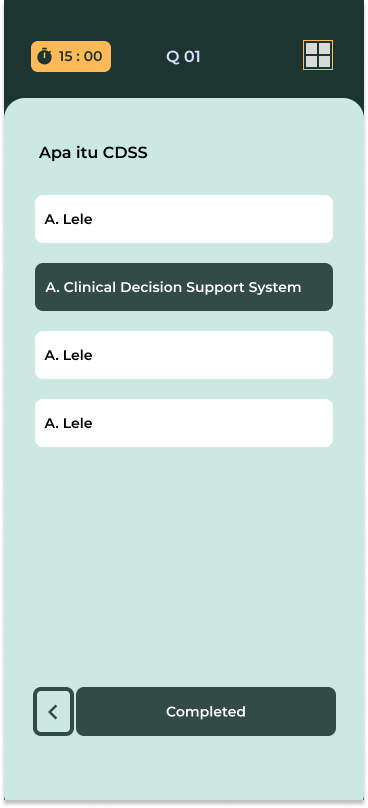
\includegraphics[width=\linewidth]{contents/chapter-3/images/HF-kuis1-dt.png}
	  \caption{Jawab kuis}
	  \label{fig:pilihJawabanDark}
	\end{subfigure}
	\begin{subfigure}[b]{0.23\textwidth}
		\centering
	  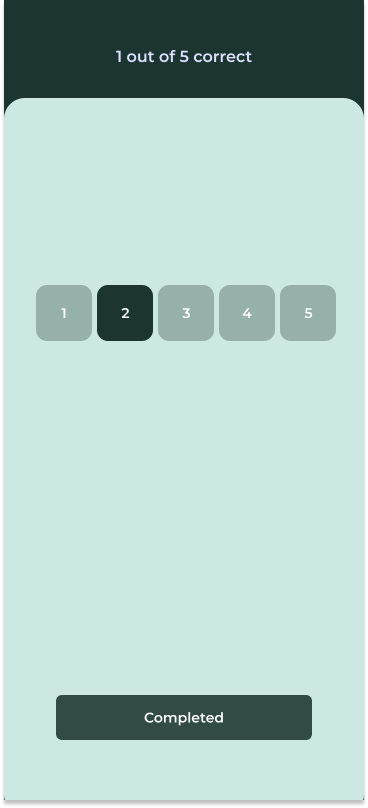
\includegraphics[width=\linewidth]{contents/chapter-3/images/HF-kuis2-dt.png}
	  \caption{\textit{Overview}}
	  \label{fig:pilihNomorDark}
	\end{subfigure}
	\begin{subfigure}[b]{0.23\textwidth}
		\centering
	  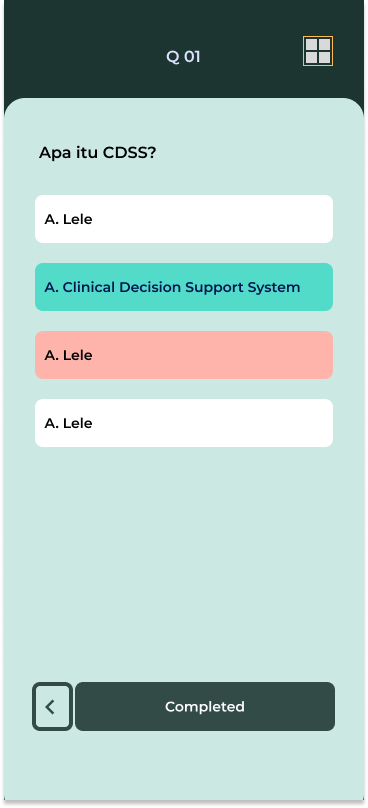
\includegraphics[width=\linewidth]{contents/chapter-3/images/HF-kuis3-dt.png}
	  \caption{\textit{Review}}
	  \label{fig:KoreksiDark}
	\end{subfigure}
	\caption{\textit{Prototype} antarmuka halaman kuis mode terang}
	\label{Fig:FeatureSetQuizDark}
\end{figure}
Untuk mode gelap pengerjaan kuis terdapat pada gambar \ref*{Fig:FeatureSetQuizDark}.
Sama seperti pada mode terang, desain terdiri dari 3 halaman yaitu jawab kuis, \textit{overview}, dan \textit{review}.
\begin{figure}[H]
	\centering
	\begin{subfigure}[b]{0.23\textwidth}
		\centering
	  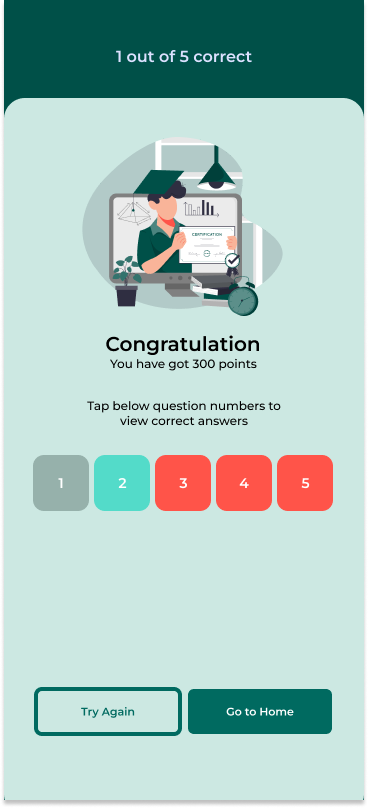
\includegraphics[width=\linewidth]{contents/chapter-3/images/HF-result.png}
	  \caption{\textit{Light Mode}}
	  \label{fig:HasilQuizResult}
	\end{subfigure}
	\begin{subfigure}[b]{0.23\textwidth}
		\centering
	  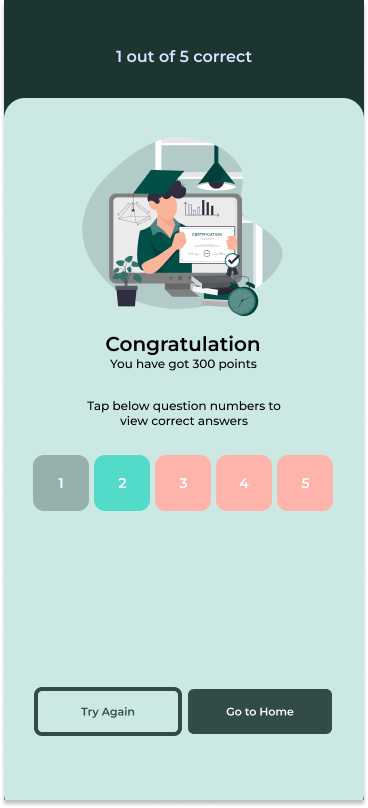
\includegraphics[width=\linewidth]{contents/chapter-3/images/HF-result-dt.png}
	  \caption{\textit{Dark Mode}}
	  \label{fig:HasilQuizResult2}
	\end{subfigure}
	\caption{\textit{Prototype} antarmuka halaman hasil kuis}
	\label{Fig:HasilFeatureSetQuizResult}
\end{figure}
Setelah mengerjakan kuis, aplikasi akan menampilkan hasil kuis yang dikerjakan. Desain hasil kuis disematkan pada gambar \ref*{Fig:HasilFeatureSetQuizResult}.

\subsection{\textit{Feature set:} Materi}
\begin{figure}[H]
	\centering
	\begin{subfigure}[b]{0.23\textwidth}
		\centering
	  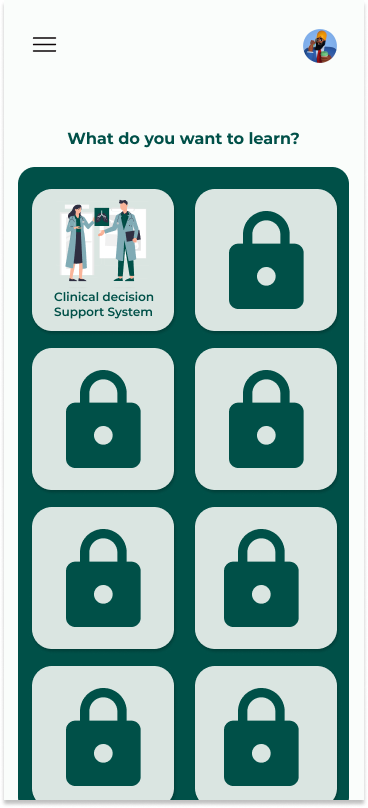
\includegraphics[width=\linewidth]{contents/chapter-3/images/HF-materi.png}
	  \caption{Halaman utama}
	  \label{fig:HasilMain2}
	\end{subfigure}
	\begin{subfigure}[b]{0.23\textwidth}
		\centering
	  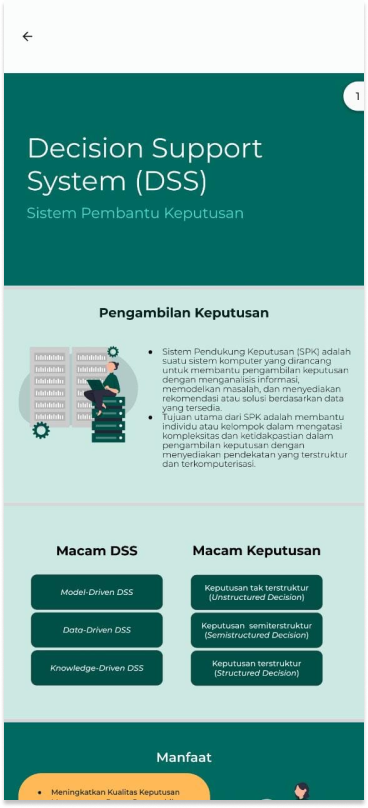
\includegraphics[width=\linewidth]{contents/chapter-3/images/HF-materi2.png}
	  \caption{\textit{Warning dialog}}
	  \label{fig:HasilMain3}
	\end{subfigure}
	\begin{subfigure}[b]{0.23\textwidth}
		\centering
	  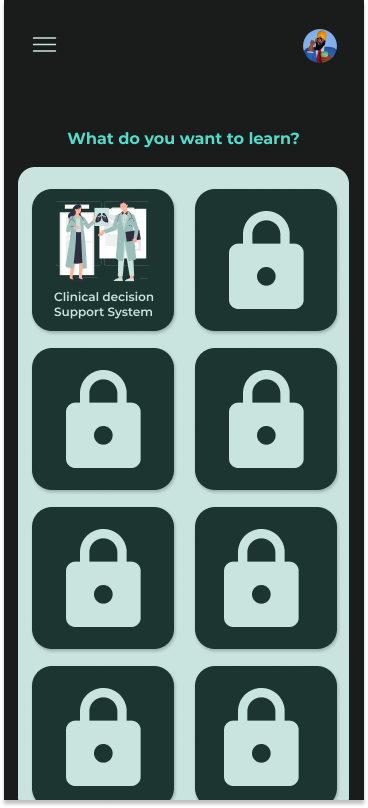
\includegraphics[width=\linewidth]{contents/chapter-3/images/HF-materi-dt.png}
	  \caption{\textit{Drawer}}
	  \label{fig:HasilMain4-dark}
	\end{subfigure}
    \begin{subfigure}[b]{0.23\textwidth}
		\centering
	  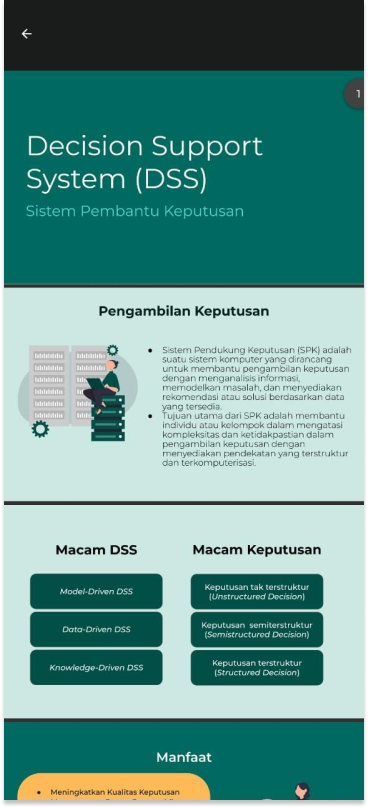
\includegraphics[width=\linewidth]{contents/chapter-3/images/HF-materi2-dt.png}
	  \caption{\textit{Drawer}}
	  \label{fig:HasilMain4}
	\end{subfigure}
	\caption{\textit{Prototype} antarmuka halaman fitur kuis}
	\label{Fig:HasilFeatureSetDrawer}
\end{figure}
Gambar \ref*{Fig:HasilFeatureSetDrawer} adalah desain dari fitur materi. Fitur ini akan menampilkan materi dalam bentuk pdf.
\subsection{\textit{Feature set: Leaderboard}}
\begin{figure}[H]
	\centering
	\begin{subfigure}[b]{0.23\textwidth}
		\centering
	  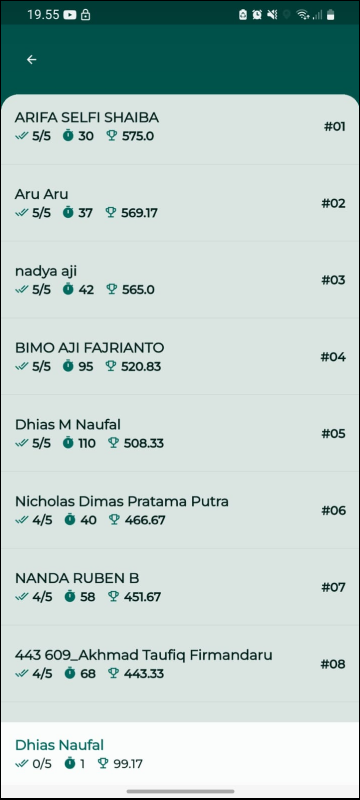
\includegraphics[width=\linewidth]{contents/chapter-3/images/HF-Leaderboard.png}
	  \caption{\textit{Light Mode}}
	  \label{fig:HasilQuizLeader}
	\end{subfigure}
	\begin{subfigure}[b]{0.23\textwidth}
		\centering
	  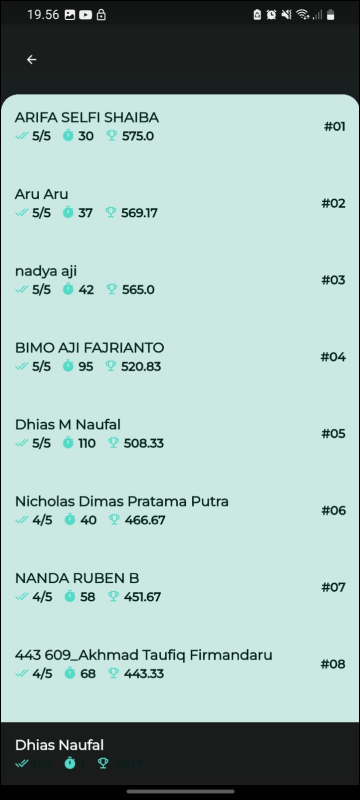
\includegraphics[width=\linewidth]{contents/chapter-3/images/HF-Leaderboard-dt.png}
	  \caption{\textit{Dark Mode}}
	  \label{fig:HasilQuizLeader2}
	\end{subfigure}
	\caption{\textit{Prototype} antarmuka halaman \textit{Leaderboard}}
	\label{Fig:HasilFeatureSetLeaderboard}
\end{figure}
Gambar \ref*{Fig:HasilFeatureSetLeaderboard} adalah desain halman \textit{Leaderboard} pada mode terang dan mode gelap.
\textit{Leaderboard} ini akan mengurutkan poin yang didapatkan per kuis yang dikerjakan.
\subsection{\textit{Feature set: Leaderboard}}
\begin{figure}[H]
	\centering
	\begin{subfigure}[b]{0.23\textwidth}
		\centering
	  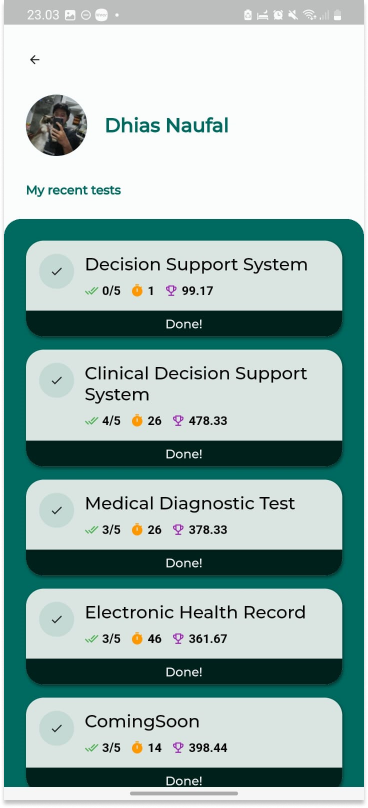
\includegraphics[width=\linewidth]{contents/chapter-3/images/HF-profil.png}
	  \caption{\textit{Light Mode}}
	  \label{fig:HasilQuizprofil}
	\end{subfigure}
	\begin{subfigure}[b]{0.23\textwidth}
		\centering
	  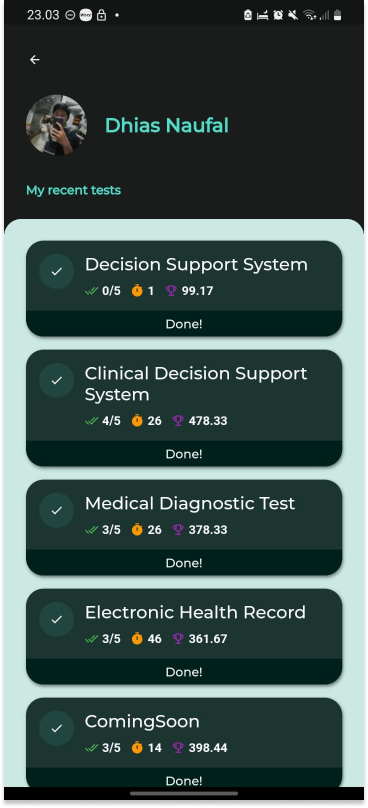
\includegraphics[width=\linewidth]{contents/chapter-3/images/HF-profil-dt.png}
	  \caption{\textit{Dark Mode}}
	  \label{fig:HasilQuizprofil2}
	\end{subfigure}
	\caption{\textit{Prototype} antarmuka halaman \textit{profile}}
	\label{Fig:HasilFeatureSetProfil}
\end{figure}
Kuis yang sudah dikerjakan akan terdaftar pada halaman profil. Daftar ini sama halnya dengan \textit{Achievement} yang didapat ketika pengguna selesai mengerjakannya.
Gambar \ref*{Fig:HasilFeatureSetProfil} adalah desain halaman profil pada mode terang dan mode gelap.
\section{Hasil Pengembangan Aplikasi}
Proses pengembangan aplikasi ini menggunakan pendekatan \textit{FDD} dimana aplikasi akan dikembangakan berdasarkan fitur yang sudah didesain.
Aplikasi yang dikembangkan ialah aplikasi \textit{android} dengan menggunakan \textit{software development kit flutter} sebagai kerangka kerjanya.
Hasil pengembangan ini memiliki indikator keberhasilan melalui pengujian fungsionalitas dari setiap fiturnya.
\subsection{Fitur \textit{Sign-in} dan \textit{Sign-out}}
\begin{table}[H]
	\centering
	\caption{\textit{Black Box Testing} fitur \textit{Sign-in} dan \textit{Sign-out}}
	\label{Tab:blackBoxSign}
	\begin{tabular}{|p{0.4\textwidth}|p{0.4\textwidth}|p{0.1\textwidth}|}
		\hline
		 \centering\textbf{Fitur} & \multicolumn{1}{m{0.45\textwidth}|}{\centering \textbf{Kriteria}}&  \multicolumn{1}{m{0.1\textwidth}|}{\centering \textbf{Hasil}}\\
		\hline
		Menampilkan halaman Sign-in 
		& Aplikasi mampu menampilkan halaman \textit{sign-in} 
		& Berhasil\\
		\hline
		Mencatat \textit{user} baru ketika melakukan \textit{Sign-in} pertama 
		& Aplikasi dapat mencatat \textit{user} baru ketika melakukan \textit{Sign-in} pertama dan mengirimkannya ke database
		& Berhasil\\
		\hline
		Aplikasi dapat memberikan akses pengguna ketika pengguna sudah terdaftar
		& Pengguna dapat menggunakan fitur aplikasi
		& Berhasil\\
		\hline
		Menghentikan pemberian akses pengguna ketika pengguna sudah terdaftar
		& Aplikasi mampu mengeluarkan akses aplikasi apda akun terkait
		& Berhasil\\
		\hline
	\end{tabular}
\end{table}
Pengujian fitur \textit{Sign-in} dan \textit{Sign-out} memiliki 4 aktivitas pengujian yang terdapat pada tabel \ref*{Fig:Black Box Testing}.
Pengujian ini medaparkan hasil 100\% berhasil untuk setiap aktivitas pengujiannya.
\subsection{Fitur \textit{Dashboard}}
\begin{table}[H]
	\centering
	\caption{\textit{Black Box Testing} fitur \textit{Dashboard}}
	\label{Tab:blackBoxDash}
	\begin{tabular}{|p{0.4\textwidth}|p{0.4\textwidth}|p{0.1\textwidth}|}
		\hline
		 \centering\textbf{Fitur} & \multicolumn{1}{m{0.45\textwidth}|}{\centering \textbf{Kriteria}}&  \multicolumn{1}{m{0.1\textwidth}|}{\centering \textbf{Hasil}}\\
		\hline
		Menampilkan halaman \textit{On Boarding} jika \textit{user} belum terdaftar 
		& Aplikasi mampu menampilkan halaman \textit{On Boarding} jika \textit{user} belum terdaftar  
		& Berhasil\\
		\hline
		Menampilkan halaman utama aplikasi
		& Ketika sudah \textit{sign-in}, penguna dapat mengakses halalman utama 
		& Berhasil\\
		\hline
		Menampilkan \textit{side drawer}
		& Aplikasi mempu menampilkan \textit{side drawer} pada sebelah kiri aplikasi
		& Berhasil\\
		\hline
		\textit{Dialog box Sign Up} jika memilih fitur, tapi \textit{user} belum terdaftar
		& Jika pengguna belum \textit{sign-in}, aplikasi menampilkan dialog box 
		& Berhasil\\
		\hline
		Memilih fitur kuis, materi, dan profil
		& Aplikasi mampu menampilkan semua fitur yang ada
		& Berhasil\\
		\hline
	\end{tabular}
\end{table}
Pengujian fitur \textit{Dashboard} memiliki 5 aktivitas pengujian yang terdapat pada tabel \ref*{Tab:blackBoxKuis}.
Pengujian ini medaparkan hasil 100\% berhasil untuk setiap aktivitas pengujiannya.
\subsection{Fitur kuis}
\begin{table}[H]
	\caption{\textit{Black Box Testing} fitur kuis}
	\label{Tab:blackBoxKuis}
	\begin{tabular}{|p{0.4\textwidth}|p{0.4\textwidth}|p{0.1\textwidth}|}
		\hline
		 \centering\textbf{Fitur} & \multicolumn{1}{m{0.45\textwidth}|}{\centering \textbf{Kriteria}}&  \multicolumn{1}{m{0.1\textwidth}|}{\centering \textbf{Hasil}}\\
		\hline
		Menampilkan halaman daftar kuis
		&  Aplikasi mampu menampilkan halaman fitur kuis yang berisi daftar kuis
		& Berhasil\\
		\hline
		Menampilkan halaman kuis yang dipilih
		& Aplikasi mampu menampilkan halaman kuis yang dipilih 
		& Berhasil\\
		\hline
		Memilih salah satu jawaban kuis berbasis pilihan ganda
		& Aplikasi mampu meilih dan menyimpan jawaban 
		& Berhasil\\
		\hline
		Menampilkkan halaman kuis nomor selanjutnya
		& Aplikasi akan menampilkan halaman kuis selanjutnya
		& Berhasil\\
		\hline
		Menampilkan halaman kuis nomor sebelumnya
		& Aplikasi akan menampilkan halaman kuis sebelumnya 
		& Berhasil\\
		\hline
		Menampilkan ringkasan kuis
		& Aplikasi akan menampilkan halaman ringkasan kuis 
		& Berhasil\\
		\hline
		Menyelesaikan kuis
		& Aplikasi dapat menutup halaman utama kuis, menghitung jawaban yang benar, dan mengirim hasilya ke database
		& Berhasil\\
		\hline
		Mendapatkan skor kuis
		& Aplikasi akan  menghitung jawaban yang benar dan menampilkan skor hasil kuis
		& Berhasil\\
		\hline
		Mencatat skor kuis
		& Aplikasi dapat mengirimkan hasil kuis ke database
		& Berhasil\\
		\hline
		Menampilkan warna merah untuk jawaban yang salah dan warna hijau untuk jawaban yang benar dalam ulasan kuis
		& Aplikasi mampu Menampilkan warna merah untuk jawaban yang salah dan warna hijau untuk jawaban yang benar dalam ulasan kuis 
		& Berhasil\\
		\hline
	\end{tabular}
\end{table}
\begin{table}[H]
	\begin{tabular}{|p{0.4\textwidth}|p{0.4\textwidth}|p{0.1\textwidth}|}
		\hline
		 \centering\textbf{Fitur} & \multicolumn{1}{m{0.45\textwidth}|}{\centering \textbf{Kriteria}}&  \multicolumn{1}{m{0.1\textwidth}|}{\centering \textbf{Hasil}}\\
		 \hline
		Memeriksa 1 per 1 jawaban kuis setelah mendapatkan skor
		& Aplikasi mampu menampilkan halaman soal kuis sesuai dengan indeks yang dipilih 
		& Berhasil\\
		\hline
		Mengerjakan kembali kuis
		& Aplikasi mampu menampilkan halaman pertama kuis dan memulai dari awal
		& Berhasil\\
		\hline
		Menutup halaman kuis dan kembali ke halaman daftar kuis
		& Aplikasi mampu menutup halaman kuis dan menampilkan halaman daftar kuis
		& Berhasil\\
		\hline
		Menutup halaman daftar kuis dan kembali ke halaman utama
		& Aplikasi mampu menutup halaman fitur daftar kuis dan kembali ke halaman utama 
		& Berhasil\\
		\hline
	\end{tabular}
\end{table}
Pengujian fitur kuis memiliki 14 aktivitas pengujian yang terdapat pada tabel \ref*{Fig:Black Box Testing}.
Pengujian ini medaparkan hasil 100\% berhasil untuk setiap aktivitas pengujiannya.
\subsection{Fitur Materi}
\begin{table}[H]
	\centering
	\caption{\textit{Black Box Testing} fitur materi}
	\label{Tab:blackBoxMateri}
	\begin{tabular}{|p{0.4\textwidth}|p{0.4\textwidth}|p{0.1\textwidth}|}
		\hline
		 \centering\textbf{Fitur} & \multicolumn{1}{m{0.45\textwidth}|}{\centering \textbf{Kriteria}}&  \multicolumn{1}{m{0.1\textwidth}|}{\centering \textbf{Hasil}}\\
		\hline
		Menampilkan halaman daftar materi yang tersedia
		& Aplikasi mampu menampilkan halaman fitur materi yang berisi daftar materi
		& Berhasil\\
		\hline
		Menampilkan materi yang dipilih
		& Aplikasi mampu menampilkan materi yang dipilih
		& Berhasil\\
		\hline
		Keluar dari materi yang dipilih
		& aplikasi mampu keluar dari aplikasi yang dipilih
		& Berhasil\\
		\hline
		Fitur kunci materi jika materi sebelumnya belum dibaca
		& Aplikasi akan mengunci file materi jika materi sebelumnya belum pernah dibuka, dan membuka jika materi seblumnya sudah pernah dibuka
		& Berhasil\\
		\hline
		Keluar dari halaman daftar materi dan kembali ke halaman utama
		& Aplikasi mampu menutup fitur materi dan kembali ke halaman utama
		& Berhasil\\
		\hline
	\end{tabular}
\end{table}
Pengujian fitur materi memiliki 4 aktivitas pengujian yang terdapat pada tabel \ref*{Fig:Black Box Testing}.
Pengujian ini medaparkan hasil 100\% berhasil untuk setiap aktivitas pengujiannya.
\subsection{Fitur Leaderboard}
\begin{table}[H]
	\caption{\textit{Black Box Testing} fitur \textit{Leaderboard}}
	\label{Tab:blackBoxLead}
	\begin{tabular}{|p{0.4\textwidth}|p{0.4\textwidth}|p{0.1\textwidth}|}
		\hline
		 \centering\textbf{Fitur} & \multicolumn{1}{m{0.45\textwidth}|}{\centering \textbf{Kriteria}}&  \multicolumn{1}{m{0.1\textwidth}|}{\centering \textbf{Hasil}}\\
		\hline
		Menampilkan halaman \textit{Leaderboard} untuk kuis yang dipilih
		&Aplikasi mampu menampilkan leaderboard untuk setiap indeks yang dipilih pada kuis 
		& Berhasil\\
		\hline
		Menampilkan hasil skor kuis pribadi yang sudah dikerjakan
		& Aplikasi menampilkan hasil skor pribadi pada halaman Leaderboard
		& Berhasil\\
		\hline
		Menampilkan urutan skor dari yang tertinggi hingga terendah
		& Aplikasi akan mengurutkan rangking pengguna berdasarkan skor kuis 
		& Berhasil\\
		\hline
		Menutup halaman leaderboard dan kembali ke halaman daftar kuis
		& Aplikasi mampu menutup halaman leaderboard dan menampilkan halaman daftar kuis
		& Berhasil\\
		\hline
	\end{tabular}
\end{table}
Pengujian fitur \textit{Leaderboard} memiliki 4 aktivitas pengujian yang terdapat pada tabel \ref*{Fig:Black Box Testing}.
Pengujian ini medaparkan hasil 100\% berhasil untuk setiap aktivitas pengujiannya.
\subsection{Fitur penghargaan}
\begin{table}[H]
	\caption{\textit{Black Box Testing} fitur \textit{Achievement}}
	\label{Tab:blackBoxAchie}
	\begin{tabular}{|p{0.4\textwidth}|p{0.4\textwidth}|p{0.1\textwidth}|}
		\hline
		 \centering\textbf{Fitur} & \multicolumn{1}{m{0.45\textwidth}|}{\centering \textbf{Kriteria}}&  \multicolumn{1}{m{0.1\textwidth}|}{\centering \textbf{Hasil}}\\
		\hline
		Menampilkan halaman profil
		& Aplikasi mampu menampilkan halaman profil 
		& Berhasil\\
		\hline
		Menampilkan penghargaan yang ada dalam halaman profil
		& Aplikasi mampu menampilkan daftar penghargaan dari kuis yang sudah dikerjakan
		& Berhasil\\
		\hline
		Menampilkan hasil scroe dari setiap kuis yang sudah dikerjakan
		& Aplikasi mampu maenampilkan hasil skor kuis dalam penghargaan kuis
		& Berhasil\\
		\hline
		Menutup halaman profil dan kembali ke halaman utama aplikasi
		&Aplikasi mampu menutup halaman profil dan menampikan halaman utama
		& Berhasil\\
		\hline
		Menghentikan pemberian akses pengguna ketika pengguna sudah terdaftar
		& Aplikasi mampu mengeluarkan akses aplikasi apda akun terkait
		& Berhasil\\
		\hline
	\end{tabular}
\end{table}
Pengujian fitur \textit{Dashboard} memiliki 4 aktivitas pengujian yang terdapat pada tabel \ref*{Fig:Black Box Testing}.
Pengujian ini medaparkan hasil 100\% berhasil untuk setiap aktivitas pengujiannya.
\newpage
\section{Analisis Hasil Pengujian}
\subsection{\textit{System Usability Scale (SUS)}}
Pengujian kegunaan dilakukan secara langsung dengan menggunakan kuesioner \textit{SUS} berbentuk \textit{Google Form}.
Pengujian kegunaan dilakukan bersamaan dengan pengujian pengalaman pengguna \textit{UEQ}.
Responden pengujian utama \textit{SUS} adalah Mahasiswa Teknik Biomedis DTETI UGM. 

Sebelum dilakukan pengujian, para responden diberikan informasi tentang aplikasi dan diminta untuk membaca dan menyetujui lembar persetujuan. 
Setelah mendapatkan persetujuan dan membaca lembar persetujuan tersebut, pengujian dimulai dengan para responden mencoba semua fitur yang tersedia dalam aplikasi MedQ, termasuk Fitur Kuis dan Fitur Materi.
Para responden diberi kebebasan untuk mencoba seluruh bagian aplikasi. Setelah mencoba semua fitur, para responden diminta untuk mengisi kuesioner SUS yang disediakan melalui Google Form. 
Pengujian ini melibatkan 38 responden, dan hasil dari kuesioner dapat dilihat dalam Tabel \ref*{Tab:SUSSKOR}
\begin{table}[H]
	\caption{Tabel skor \textit{SUS}}
	\label{Tab:SUSSKOR}
    \begin{tabular}{|>{\centering\arraybackslash}p{0.8cm}|>{\centering\arraybackslash}p{0.8cm}|>{\centering\arraybackslash}p{0.8cm}|>{\centering\arraybackslash}p{0.8cm}|>{\centering\arraybackslash}p{0.8cm}|>{\centering\arraybackslash}p{0.8cm}|>{\centering\arraybackslash}p{0.8cm}|>{\centering\arraybackslash}p{0.8cm}|>{\centering\arraybackslash}p{0.8cm}|>{\centering\arraybackslash}p{0.8cm}|>{\centering\arraybackslash}p{2cm}|}
    \hline
    Q1 & Q2 & Q3 & Q4 & Q5 & Q6 & Q7 & Q8 & Q9 & Q10 & Skor SUS    \\
    \hline
    4  & 1  & 5  & 2  & 5  & 2  & 5  & 2  & 4  & 2   & 85          \\
    \hline
    5  & 1  & 5  & 1  & 4  & 3  & 5  & 1  & 1  & 1   & 82.5        \\
    \hline
    3  & 1  & 5  & 1  & 4  & 2  & 4  & 2  & 1  & 2   & 72.5        \\
    \hline
    4  & 1  & 5  & 1  & 5  & 1  & 5  & 1  & 5  & 1   & 97.5        \\
    \hline
    4  & 1  & 5  & 1  & 4  & 2  & 5  & 1  & 3  & 3   & 82.5        \\
    \hline
    4  & 1  & 4  & 1  & 4  & 3  & 4  & 2  & 4  & 1   & 80          \\
    \hline
    4  & 3  & 5  & 3  & 4  & 2  & 4  & 2  & 5  & 3   & 72.5        \\
    \hline
    4  & 2  & 4  & 2  & 4  & 2  & 4  & 2  & 2  & 3   & 67.5        \\
    \hline
    4  & 1  & 4  & 2  & 4  & 2  & 4  & 1  & 4  & 2   & 80          \\
    \hline
    5  & 1  & 5  & 1  & 5  & 1  & 5  & 1  & 4  & 1   & 97.5        \\
    \hline
    5  & 1  & 5  & 1  & 4  & 1  & 5  & 1  & 5  & 1   & 97.5        \\
    \hline
    4  & 2  & 4  & 3  & 4  & 2  & 4  & 2  & 4  & 4   & 67.5        \\
    \hline
    4  & 2  & 4  & 2  & 4  & 2  & 4  & 2  & 4  & 4   & 70          \\
    \hline
    4  & 1  & 4  & 2  & 5  & 2  & 3  & 2  & 4  & 5   & 70          \\
    \hline
    5  & 3  & 4  & 2  & 5  & 2  & 4  & 2  & 4  & 4   & 72.5        \\
    \hline
    \end{tabular}
\end{table}
\newpage
\begin{table}[H]
    \begin{tabular}{|>{\centering\arraybackslash}p{0.8cm}|>{\centering\arraybackslash}p{0.8cm}|>{\centering\arraybackslash}p{0.8cm}|>{\centering\arraybackslash}p{0.8cm}|>{\centering\arraybackslash}p{0.8cm}|>{\centering\arraybackslash}p{0.8cm}|>{\centering\arraybackslash}p{0.8cm}|>{\centering\arraybackslash}p{0.8cm}|>{\centering\arraybackslash}p{0.8cm}|>{\centering\arraybackslash}p{0.8cm}|>{\centering\arraybackslash}p{2cm}|}
	\hline
	4  & 4  & 3  & 1  & 4  & 1  & 5  & 1  & 5  & 1   & 82.5        \\
	\hline
	2  & 2  & 4  & 2  & 3  & 3  & 4  & 3  & 4  & 4   & 57.5        \\
	\hline
	4  & 2  & 4  & 1  & 3  & 2  & 4  & 2  & 3  & 2   & 72.5        \\
	\hline
	3  & 1  & 5  & 2  & 5  & 2  & 4  & 2  & 2  & 4   & 70          \\
	\hline
	5  & 1  & 5  & 1  & 3  & 1  & 3  & 1  & 5  & 1   & 90          \\
	\hline
	4  & 2  & 5  & 5  & 5  & 2  & 4  & 1  & 5  & 4   & 72.5        \\
	\hline
	4  & 2  & 4  & 2  & 4  & 2  & 5  & 1  & 5  & 5   & 75          \\
	\hline
	4  & 3  & 3  & 4  & 4  & 4  & 3  & 3  & 3  & 4   & 47.5        \\
	\hline
	5  & 2  & 4  & 3  & 3  & 3  & 5  & 2  & 5  & 3   & 72.5        \\
	\hline
	4  & 2  & 4  & 3  & 4  & 4  & 4  & 3  & 4  & 4   & 60          \\
	\hline
	4  & 2  & 4  & 4  & 4  & 2  & 4  & 2  & 4  & 5   & 62.5        \\
	\hline
	5  & 1  & 5  & 1  & 5  & 2  & 4  & 2  & 4  & 1   & 90          \\
	\hline
	3  & 1  & 5  & 1  & 4  & 2  & 5  & 1  & 4  & 2   & 85          \\
	\hline
	3  & 1  & 4  & 1  & 4  & 2  & 4  & 1  & 4  & 2   & 80          \\
    \hline
    5  & 1  & 5  & 4  & 2  & 2  & 5  & 1  & 2  & 2   & 72.5        \\
    \hline
    5  & 1  & 5  & 2  & 5  & 2  & 5  & 1  & 5  & 1   & 95          \\
    \hline
    5  & 2  & 5  & 1  & 5  & 1  & 5  & 1  & 5  & 3   & 92.5        \\
    \hline
    4  & 4  & 3  & 2  & 4  & 1  & 3  & 2  & 4  & 2   & 67.5        \\
    \hline
    4  & 1  & 5  & 2  & 3  & 1  & 5  & 2  & 3  & 4   & 75          \\
    \hline
    5  & 2  & 4  & 1  & 5  & 2  & 5  & 2  & 5  & 3   & 85          \\
    \hline
    4  & 2  & 4  & 4  & 4  & 1  & 3  & 3  & 4  & 3   & 65          \\
    \hline
    3  & 3  & 2  & 2  & 4  & 4  & 2  & 4  & 2  & 5   & 37.5        \\
    \hline
    2  & 3  & 3  & 4  & 3  & 3  & 3  & 3  & 4  & 5   & 42.5        \\
    \hline
    \multicolumn{10}{|l|}{Rata-rata skor SUS} & 74.9 \\
    \hline
    \end{tabular}
\end{table}
Data hasil kuesioner SUS kemudian diolah menggunakan persamaan \ref*{Perhitungan rata-rata skor SUS} yang dijelaskan pada bab II untuk menghasilkan skor SUS untuk setiap responden. Selanjutnya, seluruh skor SUS dijumlahkan dan dihitung rata-ratanya. Aplikasi MedQ memperoleh rata-rata skor SUS sebesar 74,9, yang menunjukkan bahwa aplikasi MedQ masuk dalam kategori "Good" berdasarkan klasifikasi skor rata-rata yang tercantum dalam Tabel  \ref*{Tabel pertanyaan kuesioner sus} di bab II. Dapat disimpulkan bahwa secara kegunaan aplikasi MEDQ layak dan dapat diterima. 
pada bab II menurut Bangor et al. Dengan demikian, dapat disimpulkan bahwa aplikasi MedQ layak dan dapat diterima dalam hal kegunaannya.
\newpage
\subsection{\textit{User Experience Questionnaire (UEQ)}}
Pengujian pengalaman pengguna dilakukan secara langsung dengan menggunakan kuesioner \textit{UEQ} berbentuk \textit{Google Form}.
Pengujian pengalaman pengguna bersamaan dengan pengujian\textit{SUS}.
Responden pengujian pengalaman pengguna adalah Mahasiswa Teknik Biomedis DTETI UGM. 

Data hasil kuesioner UEQ diolah menggunakan UEQ Data Analysis Tool versi 12 yang tersedia di ueqonline.org oleh Martin Schrepp, pencipta UEQ. 
Tahap awal dalam pengolahan data UEQ adalah melakukan pemeriksaan terhadap data yang tidak valid. 
Dari total 38 responden, terdapat 4 data yang bermasalah (dengan ciri kolom warna merah) karena memiliki nilai \textit{"critical"} atau lebih, sebagaimana ditampilkan pada gambar \ref*{Fig:InvalidUEQ}. 
Keempat data tersebut dianggap tidak valid, karena mungkin disebabkan oleh respon acak atau kesalahpahaman dalam memahami pertanyaan. 
Oleh karena itu, keempat data tersebut harus dihapus dari perhitungan UEQ.
\begin{figure}[H]
	\centering
	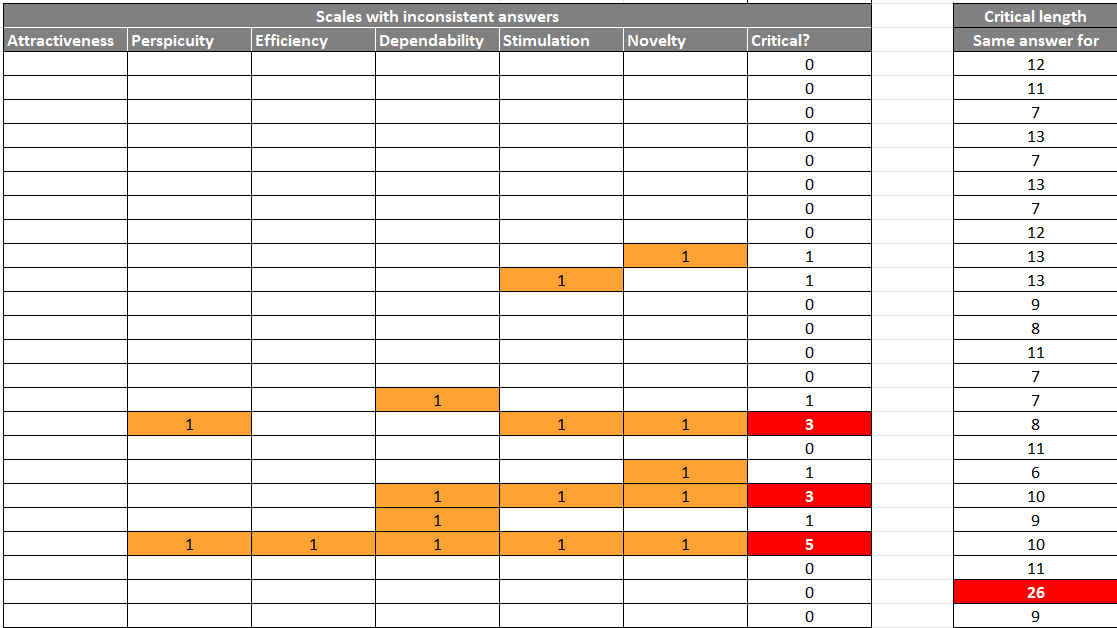
\includegraphics[width=0.8\textwidth]{contents/chapter-4/images/invalidUEQ.png}
	\caption{Data invalid pada UEQ}
	\label{Fig:InvalidUEQ}
\end{figure}

Hasil rata-rata skala UEQ tiap aspek pengalaman pengguna untuk Aplikasi 
MedQ dipaparkan dalam tabel pada gambar \ref*{Fig : Tabel Skor UEQ} dan grafik pada gambar \ref*{Fig : Gambar Skor UEQ }.
\begin{figure}[H]
	\centering
	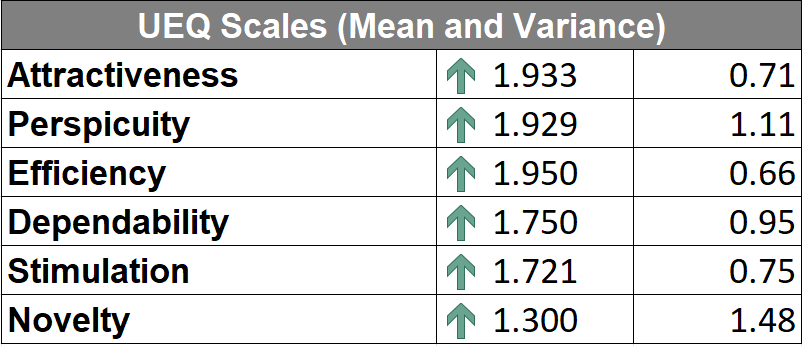
\includegraphics[width=0.6\textwidth]{contents/chapter-4/images/UEQScore.png}
	\caption{\textit{benchmark} hasil \textit{UEQ}}
	\label{Fig : Tabel Skor UEQ}
\end{figure}
\begin{figure}[H]
	\centering
	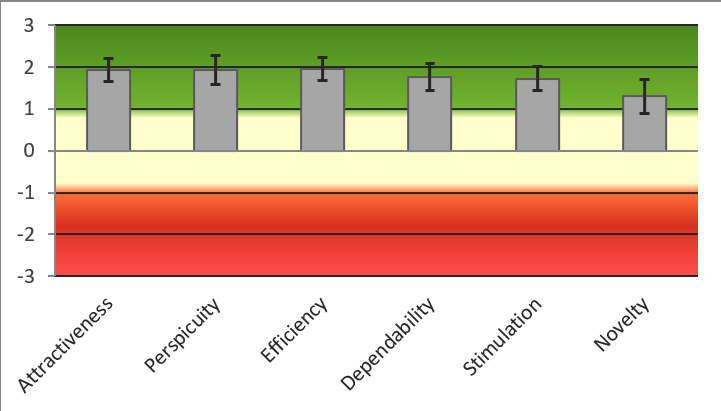
\includegraphics[width=0.7\textwidth]{contents/chapter-4/images/UEQScore-graph.png}
	\caption{\textit{benchmark} hasil \textit{UEQ}}
	\label{Fig : Gambar Skor UEQ }
\end{figure}

Aplikasi MedQ mendapat nilai rata-rata 1,93 untuk skala daya tarik atau 
Attractiveness, mendapat nilai rata-rata 1,93 untuk skala kejelasan atau 
Perspicuity dan mendapat nilai ra-rata 1,95 untuk skala efisiensi. Untuk skala 
ketepatan atau \textit{Dependability} aplikasi MedQ mendapat nilai rata-rata 1,75 dan 
mendapat nilai rata-rata 1,72 untuk skala stimulasi. Sedangkan untuk skala 
kebaruan aplikasi MedQ mendapat nilai rata-rata 1,3. 
\begin{figure}[H]
	\centering
	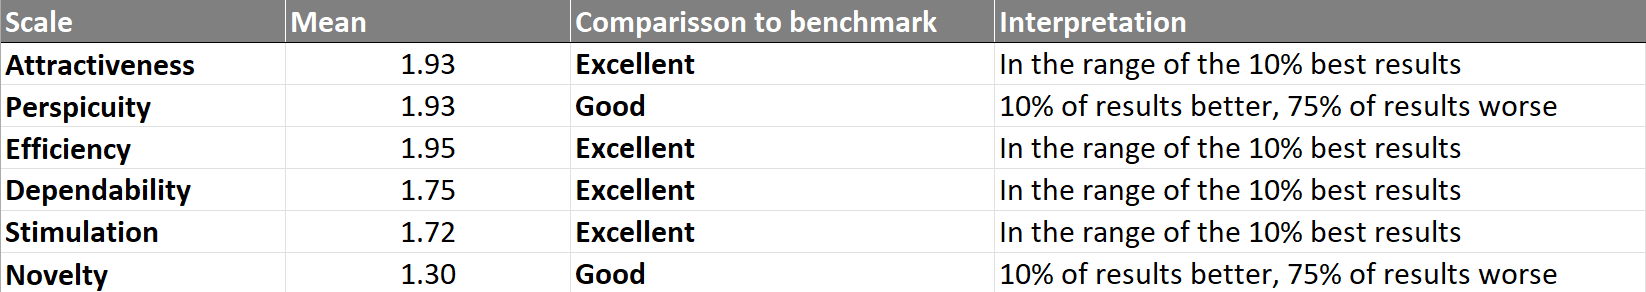
\includegraphics[width=0.9\textwidth]{contents/chapter-4/images/BenchMark.png}
	\caption{\textit{benchmark} hasil \textit{UEQ}}
	\label{Fig : benchmark}
\end{figure}
\begin{figure}[H]
	\centering
	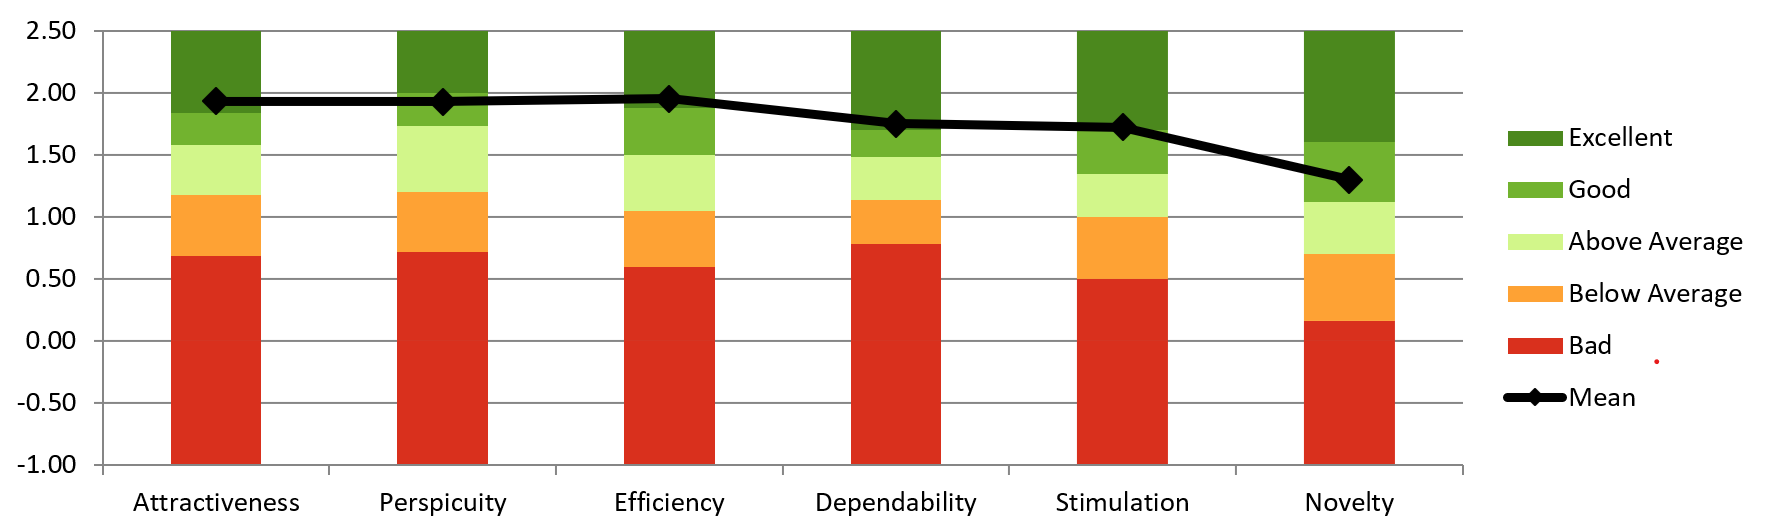
\includegraphics[width=0.8\textwidth]{contents/chapter-4/images/BenchMark-graph.png}
	\caption{\textit{benchmark} hasil \textit{UEQ}}
	\label{Fig : benchmark-graph}
\end{figure}
Apabila dibandingkan dengan benchmark maka aplikasi MedQ masuk ke 
dalam kategori \textit{Excellent} untuk skala daya tarik, efisiensi, ketepatanm dan stimulasi.
Tapi masuk kategori \textit{Good} untuk skala kejelasan dan kebaruan